
%\tikzset{->,>=stealth'}
\begin{figure}[H]
\vspace{-25pt}
%\begin{wrapfigure}[10]{L}{0.45\textwidth}
%\begin{cutout}{2}{0pt}{\dimexpr0.4\linewidth\relax}{6}
%  \begin{center}
  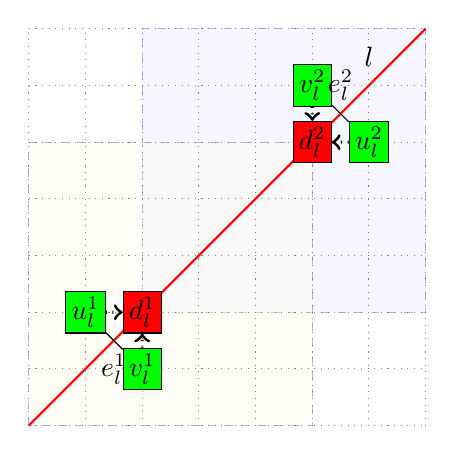
\begin{tikzpicture}[scale=0.36]
    \draw[blue, dashed, fill=blue!10, opacity=0.3] (4,4) -- (4,14) -- (14,14) -- (14,4) -- cycle; 
    \draw[blue, dashed, fill=yellow!10, opacity=0.3] (0,0) -- (0,10) -- (10,10) -- (10,0) -- cycle; 
    \draw[color=gray, style=dotted] (0,0)  
      grid[xstep=2cm, ystep=2cm] (14cm,14cm);
  	% \node at (4,5) [draw,fill=green,inner sep=0pt,minimum size=1pt] {\scriptsize $u^1_l$};
  	\node(u1l) at (2,4) [draw,fill=green,inner sep=2pt] {$u^1_l$};
  	\node(v1l) at (4,2) [draw,fill=green,inner sep=2pt] {$v^1_l$};
	\draw[red,thick] (0,0) -- (14,14); 
    \node(d1l) at (4,4) [draw,fill=red,inner sep=2pt] {$d_l^1$};
    \node(d2l) at (10,10) [draw,fill=red,inner sep=2pt] {$d_l^2$};
    \node(v2l) at (10,12) [draw, fill=green, inner sep=2pt] {$v^2_l$};
    \node(u2l) at (12,10) [draw, fill=green, inner sep=2pt] {$u^2_l$};
    \node at (12,13) [draw=none] {$l$};
    \node at (3,2) [draw=none] {$e_l^1$};
    \node at (11,12) [draw=none] {$e_l^2$};
    \draw(u1l) to (v1l);
    \draw(v2l) to (u2l);
    \draw[color=black, style=dotted] (v1l) edge[line width=1.1pt,->] (d1l);    
    \draw[color=black, style=dotted] (u1l) edge[line width=1.1pt,->] (d1l);
    \draw[color=black, style=dotted] (v2l) edge[line width=1.1pt,->] (d2l);
    \draw[color=black, style=dotted] (u2l) edge[line width=1.1pt,->] (d2l);
  \end{tikzpicture}
  \caption{Green vertices belong to the graph, red vertices  do not belong to the graph. From the dotted arrows we will choose $2$ to compensate for the gap line $l$.}
  \label{key_lemma_pic}
%  \end{center}
%\end{cutout}
%\end{wrapfigure}
  \end{figure}
